\begin{figure}
  \centering 
  \begin{subfigure}[b]{6.0cm}
    \centering
    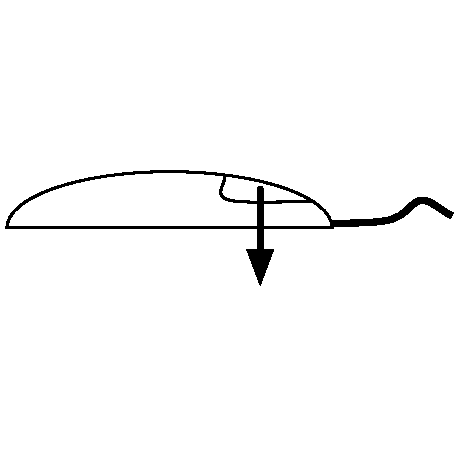
\includegraphics[origin=c, width=\textwidth]{img/button-force-mouse.pdf} 
    \caption{Force vector for mouse button press is perpendicular to
      the plane the device rests on. It will therefore not move much.}
    \label{fig:button-force-mouse} 
  \end{subfigure}
  \hspace{0.5cm} 
  \begin{subfigure}[b]{6.0cm}
    \centering
    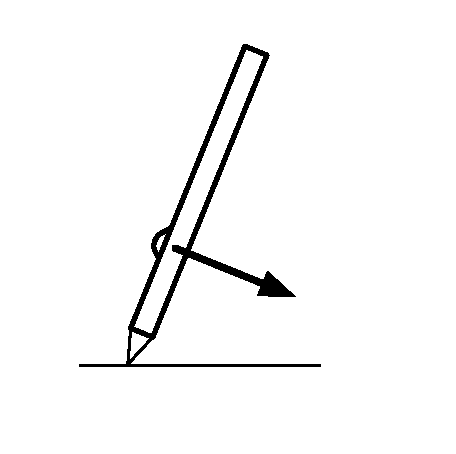
\includegraphics[origin=c, width=\textwidth]{img/button-force-pen.pdf} 
    \caption{Pressing a stylus button is more likely to cause unwanted
      pen tip movement because it is at an acute angle to the drawing
      surface plane.}
    \label{fig:button-force-pen} 
  \end{subfigure}
  \caption[Pen vs. Mouse]{The force required to press a mouse button compared with a
    stylus button.}
  \label{fig:button-force}
\end{figure}
